\documentclass[journal,12pt,twocolumn]{IEEEtran}
%\usepackage{chngcntr}
\usepackage{setspace}
\usepackage{float}
\usepackage{gensymb}
\singlespacing
% \usepackage[cmex10]{amsmath}
\usepackage{caption}
\usepackage{epstopdf}
\usepackage[cmex10]{amsmath}
\usepackage{amsthm}
%\interdisplaylinepenalty=2500
%\savesymbol{iint}
%\usepackage{txfonts}
%\restoresymbol{TXF}{iint}
%\usepackage{wasysym}
\usepackage{amsthm}
%\usepackage{iithtlc}
\usepackage{mathrsfs}
\usepackage{txfonts}
\usepackage[utf8]{inputenc}
\usepackage{float}
\usepackage{listings}
\usepackage{bm}
\usepackage{mathptmx}
\usepackage{amsfonts}
\usepackage{subfig}
\usepackage{xtab}
\usepackage{longtable}

%\usepackage{algorithm}
%\usepackage{algpseudocode}
%\usepackage{chngcntr}




\usepackage{mathrsfs}
\usepackage{txfonts}
\usepackage{stfloats}
\usepackage{bm}
\usepackage{cite}
% \usepackage{cases}
\usepackage{subfig}

\usepackage{longtable}
% \usepackage{multirow}

\usepackage{enumitem}
\usepackage{mathtools}
% \usepackage{steinmetz}
\usepackage{tikz}
%\usepackage{circuitikz}
\usepackage{verbatim}
% \usepackage{tfrupee}
\usepackage[breaklinks=true]{hyperref}
\usepackage{graphicx}
% \usepackage{tkz-euclide}

\usetikzlibrary{calc,math}
\usepackage{listings}
    \usepackage{color}                                            %%
    \usepackage{array}                                            %%
    \usepackage{longtable}                                        %%
    \usepackage{calc}                                             %%
    %\usepackage{multirow}                                         %%
    \usepackage{hhline}                                           %%
    \usepackage{ifthen}                                           %%
    \usepackage{lscape}     
\usepackage{multicol}
\usepackage{chngcntr}
\usepackage{xcolor}
%\DeclareMathOperator*{\Res}{Res}

\renewcommand\thesection{\arabic{section}}
\renewcommand\thesubsection{\thesection.\arabic{subsection}}
\renewcommand\thesubsubsection{\thesubsection.\arabic{subsubsection}}

\renewcommand\thesectiondis{\arabic{section}}
\renewcommand\thesubsectiondis{\thesectiondis.\arabic{subsection}}
\renewcommand\thesubsubsectiondis{\thesubsectiondis.\arabic{subsubsection}}
\newcommand\myText[1]{\text{\scriptsize\tabular[t]{@{}l@{}}#1\endtabular}}

\hyphenation{op-tical net-works semi-conduc-tor}
\def\inputGnumericTable{}                                 %%

\lstset{
%language=C,
frame=single, 
breaklines=true,
columns=fullflexible
}
\begin{document}


\newtheorem{theorem}{Theorem}[section]
\newtheorem{problem}{Problem}
\newtheorem{proposition}{Proposition}[section]
\newtheorem{lemma}{Lemma}[section]
\newtheorem{corollary}[theorem]{Corollary}
\newtheorem{example}{Example}[section]
\newtheorem{definition}[problem]{Definition}

\newcommand{\BEQA}{\begin{eqnarray}}
\newcommand{\EEQA}{\end{eqnarray}}
\newcommand{\define}{\stackrel{\triangle}{=}}
\bibliographystyle{IEEEtran}
\raggedbottom
\setlength{\parindent}{0pt}
\providecommand{\mbf}{\mathbf}
\providecommand{\pr}[1]{\ensuremath{\Pr\left(#1\right)}}
\providecommand{\qfunc}[1]{\ensuremath{Q\left(#1\right)}}
\providecommand{\sbrak}[1]{\ensuremath{{}\left[#1\right]}}
\providecommand{\lsbrak}[1]{\ensuremath{{}\left[#1\right.}}
\providecommand{\rsbrak}[1]{\ensuremath{{}\left.#1\right]}}
\providecommand{\brak}[1]{\ensuremath{\left(#1\right)}}
\providecommand{\lbrak}[1]{\ensuremath{\left(#1\right.}}
\providecommand{\rbrak}[1]{\ensuremath{\left.#1\right)}}
\providecommand{\cbrak}[1]{\ensuremath{\left\{#1\right\}}}
\providecommand{\lcbrak}[1]{\ensuremath{\left\{#1\right.}}
\providecommand{\rcbrak}[1]{\ensuremath{\left.#1\right\}}}
\theoremstyle{remark}
\newtheorem{rem}{Remark}
\newcommand{\sgn}{\mathop{\mathrm{sgn}}}
\providecommand{\abs}[1]{\left\vert#1\right\vert}
\providecommand{\res}[1]{\Res\displaylimits_{#1}} 
\providecommand{\norm}[1]{\left\lVert#1\right\rVert}
%\providecommand{\norm}[1]{\lVert#1\rVert}
\providecommand{\mtx}[1]{\mathbf{#1}}
\providecommand{\mean}[1]{E\left[ #1 \right]}
\providecommand{\fourier}{\overset{\mathcal{F}}{ \rightleftharpoons}}
%\providecommand{\hilbert}{\overset{\mathcal{H}}{ \rightleftharpoons}}
\providecommand{\system}{\overset{\mathcal{H}}{ \longleftrightarrow}}
	%\newcommand{\solution}[2]{\textbf{Solution:}{#1}}
\newcommand{\solution}{\noindent \textbf{Solution: }}
\newcommand{\cosec}{\,\text{cosec}\,}
\providecommand{\dec}[2]{\ensuremath{\overset{#1}{\underset{#2}{\gtrless}}}}
\newcommand{\myvec}[1]{\ensuremath{\begin{pmatrix}#1\end{pmatrix}}}
\newcommand{\mydet}[1]{\ensuremath{\begin{vmatrix}#1\end{vmatrix}}}
%\numberwithin{equation}{subsection}

\makeatletter
\@addtoreset{figure}{problem}
\makeatother
\let\StandardTheFigure\thefigure
\let\vec\mathbf

\renewcommand{\thefigure}{\theproblem}

\def\putbox#1#2#3{\makebox[0in][l]{\makebox[#1][l]{}\raisebox{\baselineskip}[0in][0in]{\raisebox{#2}[0in][0in]{#3}}}}
     \def\rightbox#1{\makebox[0in][r]{#1}}
     \def\centbox#1{\makebox[0in]{#1}}
     \def\topbox#1{\raisebox{-\baselineskip}[0in][0in]{#1}}
     \def\midbox#1{\raisebox{-0.5\baselineskip}[0in][0in]{#1}}
\vspace{3cm}
\title{Assignment 1}
\author{G Yashwanth Naik - EE18BTECH11017}
\maketitle
\newpage
\bigskip
\renewcommand{\thefigure}{\theenumi}
\renewcommand{\thetable}{\theenumi}



Download all python codes from 
\begin{lstlisting}
https://github.com/yashwanthguguloth24/EE3025-DSP-lab/tree/main/Assignment1/codes
\end{lstlisting}
%
and latex-tikz codes from 
%
\begin{lstlisting}
https://github.com/yashwanthguguloth24/EE3025-DSP-lab/tree/main/Assignment1
\end{lstlisting}


\section{Problem}
\begin{enumerate}[label=\thesection.\arabic*.,ref=\thesection.\theenumi]
    \numberwithin{equation}{enumi}
    
    \item Let
    \begin{align}
        x(n) = \cbrak{\underset{\uparrow}{1},2,3,4,2,1}
         \label{eq:equation0}\\
        y(n) + \frac{1}{2}y(n-1) = x(n) + x(n-2)	
        \label{eq:equation1}
    \end{align}
    
    \item Compute 
    \begin{align}
        X(k) \triangleq \sum_{n=0}^{N-1} x(n) e^{-j 2 \pi k n / N}, \quad k=0,1, \ldots, N-1
    \end{align}
    and $H(k)$ using h(n).
    
    \item Compute 
    \begin{align}
    Y(k) = X(k)H(k)
    \end{align}

\end{enumerate}

\section{Solution}
\begin{enumerate}[label=\thesection.\arabic*.,ref=\thesection.\theenumi]
\numberwithin{equation}{enumi}
\item
We know that,the Impulse Response of the LTI system is the output of the system when Unit Impulse Signal is given as input to the system.
\newline
So, using Eq \eqref{eq:equation1} the Impulse Response of the System can be found as,
\begin{align}
    h(n) + \frac{1}{2}h(n-1) = \delta(n) + \delta(n-2)	
\end{align}
where $h(n)$ is an IIR Filter.
\item DFT of a Input Signal $x(n)$ is 
\begin{align}
    X(k) \triangleq \sum_{n=0}^{N-1} x(n) e^{-j 2 \pi k n / N}, \quad k=0,1, \ldots, N-1
\end{align}

For N = 6, The above expression can be written in matrix form as below:
\begin{equation}
\renewcommand{\arraystretch}{1.45}
\setlength\arraycolsep{0.01pt}
\begin{bmatrix} 
X(0) \\ X(1) \\ X(2) \\ X(3) \\ X(4) \\ X(5) 
\end{bmatrix}
=
\begin{bmatrix}
W^{0}_{6} & W^{0}_{6} & W^{0}_{6} & W^{0}_{6} & W^{0}_{6} & W^{0}_{6}\\
W^{0}_{6} & W^{1}_{6} & W^{2}_{6} & W^{3}_{6} & W^{4}_{6} & W^{5}_{6}\\
W^{0}_{6} & W^{2}_{6} & W^{4}_{6} & W^{6}_{6} & W^{8}_{6} & W^{10}_{6}\\
W^{0}_{6} & W^{3}_{6} & W^{6}_{6} & W^{9}_{6} & W^{12}_{6} & W^{15}_{6}\\
W^{0}_{6} & W^{4}_{6} & W^{8}_{6} & W^{12}_{6} & W^{16}_{6} & W^{20}_{6}\\
W^{0}_{6} & W^{5}_{6} & W^{10}_{6} & W^{15}_{6} & W^{20}_{6} & W^{25}_{6} 
\end{bmatrix}
\begin{bmatrix}
x(1) \\ x(2) \\ x(3) \\ x(4) \\ x(5) \\x(6)
\end{bmatrix}
\end{equation}

Where $W_{N} = e^{-j2\pi/N}$
\begin{align}
\implies W_{6} = e^{-j2\pi/6} = \frac{1-j\sqrt{3}}{2}
\end{align}
\newline
Using $x(n)$ from Eq\eqref{eq:equation0}, we get
\begin{equation}
\renewcommand{\arraystretch}{1.45}
\setlength\arraycolsep{0.01pt}
\begin{bmatrix} 
X(0) \\ X(1) \\ X(2) \\ X(3) \\ X(4) \\ X(5) 
\end{bmatrix}
=
\begin{bmatrix}
W^{0}_{6} & W^{0}_{6} & W^{0}_{6} & W^{0}_{6} & W^{0}_{6} & W^{0}_{6}\\
W^{0}_{6} & W^{1}_{6} & W^{2}_{6} & W^{3}_{6} & W^{4}_{6} & W^{5}_{6}\\
W^{0}_{6} & W^{2}_{6} & W^{4}_{6} & W^{6}_{6} & W^{8}_{6} & W^{10}_{6}\\
W^{0}_{6} & W^{3}_{6} & W^{6}_{6} & W^{9}_{6} & W^{12}_{6} & W^{15}_{6}\\
W^{0}_{6} & W^{4}_{6} & W^{8}_{6} & W^{12}_{6} & W^{16}_{6} & W^{20}_{6}\\
W^{0}_{6} & W^{5}_{6} & W^{10}_{6} & W^{15}_{6} & W^{20}_{6} & W^{25}_{6} 
\end{bmatrix}
\begin{bmatrix}
1 \\ 2 \\ 3 \\ 4 \\ 2 \\ 1
\end{bmatrix}
\end{equation}


On simplifying we get,
\begin{align}
    \renewcommand{\arraystretch}{1.35}
    \begin{bmatrix} X(0) \\ X(1) \\ X(2) \\ X(3) \\ X(4) \\ X(5) \end{bmatrix}
=
\begin{bmatrix}
1 +2+3+4+2+1 \\ 1+ (2)e^{-j\pi /3} + ... + (1)e^{-j5\pi /3}\\ 1 + (2)e^{-2j\pi /3} + ... +(1)(e^{-2j5\pi /3}\\ 1 + (2)e^{-3j\pi /3} + ... + (1)e^{-3j5\pi /3}\\ 1 + (2)e^{-4j\pi /3} + ... + (1)e^{-4j5\pi /3}\\ 1 + (2)e^{-5j\pi /3} + ... + (1)e^{-5j5\pi /3}
\end{bmatrix}
\end{align}

Finally,
\begin{equation}
\renewcommand{\arraystretch}{1.35}
\setlength\arraycolsep{0.01pt}
\begin{bmatrix} 
X(0) \\ X(1) \\ X(2) \\ X(3) \\ X(4) \\ X(5) 
\end{bmatrix}
=
\begin{bmatrix}
13+0j \\ -4-1.732j \\ 1+0j  \\ -1+0j \\ 1+0j \\ -4+1.732j
\end{bmatrix}
\end{equation}


\item DFT of a Impulse Response $h(n)$ is 
\begin{align}
    H(k) \triangleq \sum_{n=0}^{N-1} h(n) e^{-j 2 \pi k n / N}, \quad k=0,1, \ldots, N-1
\end{align}
Similarly, converting the above expression in matrix form to find $H(k)$
\begin{equation}
\renewcommand{\arraystretch}{1.45}
\setlength\arraycolsep{0.01pt}
\begin{bmatrix} 
H(0) \\ H(1) \\ H(2) \\ H(3) \\ H(4) \\ H(5) 
\end{bmatrix}
=
\begin{bmatrix}
W^{0}_{6} & W^{0}_{6} & W^{0}_{6} & W^{0}_{6} & W^{0}_{6} & W^{0}_{6}\\
W^{0}_{6} & W^{1}_{6} & W^{2}_{6} & W^{3}_{6} & W^{4}_{6} & W^{5}_{6}\\
W^{0}_{6} & W^{2}_{6} & W^{4}_{6} & W^{6}_{6} & W^{8}_{6} & W^{10}_{6}\\
W^{0}_{6} & W^{3}_{6} & W^{6}_{6} & W^{9}_{6} & W^{12}_{6} & W^{15}_{6}\\
W^{0}_{6} & W^{4}_{6} & W^{8}_{6} & W^{12}_{6} & W^{16}_{6} & W^{20}_{6}\\
W^{0}_{6} & W^{5}_{6} & W^{10}_{6} & W^{15}_{6} & W^{20}_{6} & W^{25}_{6}  
\end{bmatrix}
\begin{bmatrix}
h(1) \\ h(2) \\ h(3) \\ h(4) \\ h(5) \\ h(6)
\end{bmatrix}
\end{equation}


Further Simplification we get,
\begin{align}
    \renewcommand{\arraystretch}{1.35}
    \begin{bmatrix} H(0) \\ H(1) \\ H(2) \\ H(3) \\ H(4) \\ H(5) \end{bmatrix}
=
\begin{bmatrix}
h(0) + h(1) + h(2) + h(3) + h(4) + h(5) \\h(0) + h(1)e^{-j\pi /3} + ... + h(5)e^{-j5\pi /3}\\h(0) + h(1)e^{-2j\pi /3} + ... + h(5)e^{-2j5\pi /3}\\h(0) + h(1)e^{-3j\pi /3} + ... + h(5)e^{-3j5\pi /3}\\
h(0) + h(1)e^{-4j\pi /3} + ... + h(5)e^{-4j5\pi /3}\\h(0) + h(1)e^{-5j\pi /3} + ... + h(5)e^{-5j5\pi /3}
\end{bmatrix}
\end{align}



Finally we get,
\begin{equation}
\renewcommand{\arraystretch}{1.45}
\setlength\arraycolsep{0.01pt}
\begin{bmatrix} 
H(0) \\ H(1) \\ H(2) \\ H(3) \\ H(4) \\ H(5) 
\end{bmatrix}
=
\begin{bmatrix}
1.28125+0j \\ 0.51625-0.51418j \\ -0.07812+1.10956j  \\ 3.84375+0j \\ -0.07182-1.10956j \\ 0.51625+0.51418j
\end{bmatrix}
\end{equation}



\item The magnitude and phase plots of $X(k)$ and $H(k)$
\begin{figure}[!ht]
	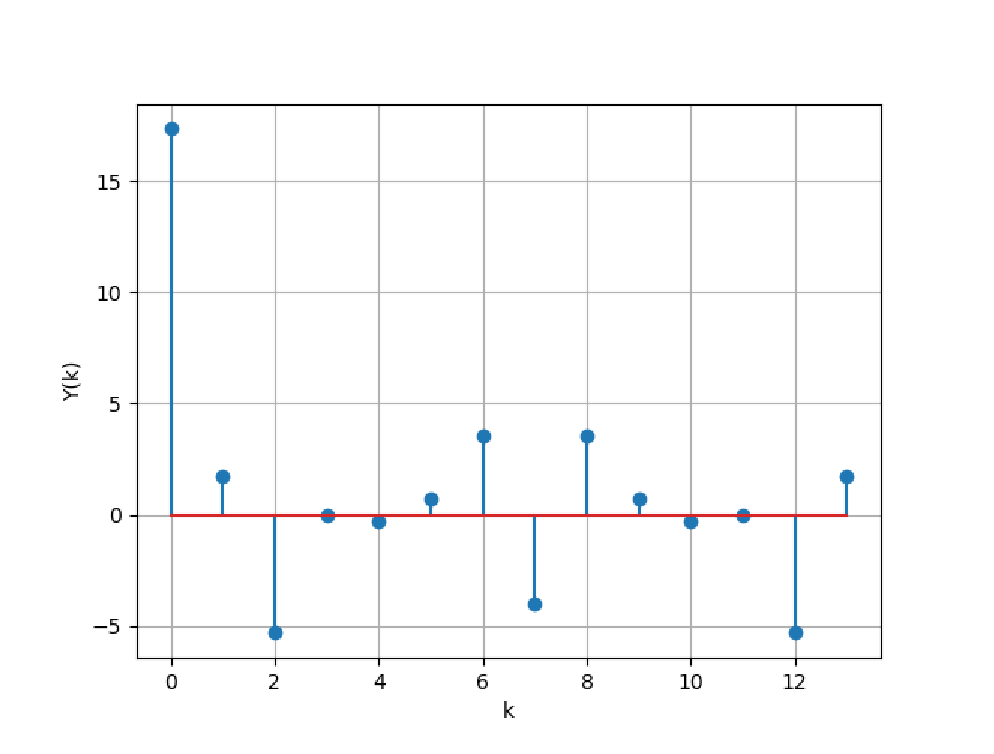
\includegraphics[width=1.15\columnwidth]{./figs/ee18btech11017_fig1.eps}
\end{figure}

\item We can now compute $Y(k)$ using 	Eq \eqref{eq:equation2}

\begin{align}
    Y(k) = X(k)H(k)
    \label{eq:equation2}
\end{align}

So, $Y(k)$ is obtained element wise multiplication of $X(k)$ and $H(k)$
\begin{equation}
\renewcommand{\arraystretch}{1.45}
\setlength\arraycolsep{0.01pt}
\begin{bmatrix} 
Y(0) \\ Y(1) \\ Y(2) \\ Y(3) \\ Y(4) \\ Y(5) 
\end{bmatrix}
=
\begin{bmatrix}
X(0)\cdot H(0) \\ X(1)\cdot H(1) \\ X(2)\cdot H(2) \\ X(3)\cdot H(3) \\ X(4)\cdot H(4) \\ X(5)\cdot H(5)
\end{bmatrix}
\end{equation}

Computing the above expression we get,
\begin{equation}
\renewcommand{\arraystretch}{1.45}
\setlength\arraycolsep{0.01pt}
\begin{bmatrix} 
Y(0) \\ Y(1) \\ Y(2) \\ Y(3) \\ Y(4) \\ Y(5) 
\end{bmatrix}
=
\begin{bmatrix}
16.6562+0j \\ -2.95312+1.16372j \\ -0.07812+1.10959j \\ -3.84375-9.27556j \\ -0.07812-1.10959j \\ -2.95312-1.16372j 
\end{bmatrix}
\end{equation}


%[16.65625 +0.00000000e+00j -2.953125+1.16372164e+00j
% -0.078125+1.10959505e+00j -3.84375 -9.27556643e-15j
% -0.078125-1.10959505e+00j -2.953125-1.16372164e+00j]

The magnitude and phase plots of $Y(k)$ are
\begin{figure}[!ht]
	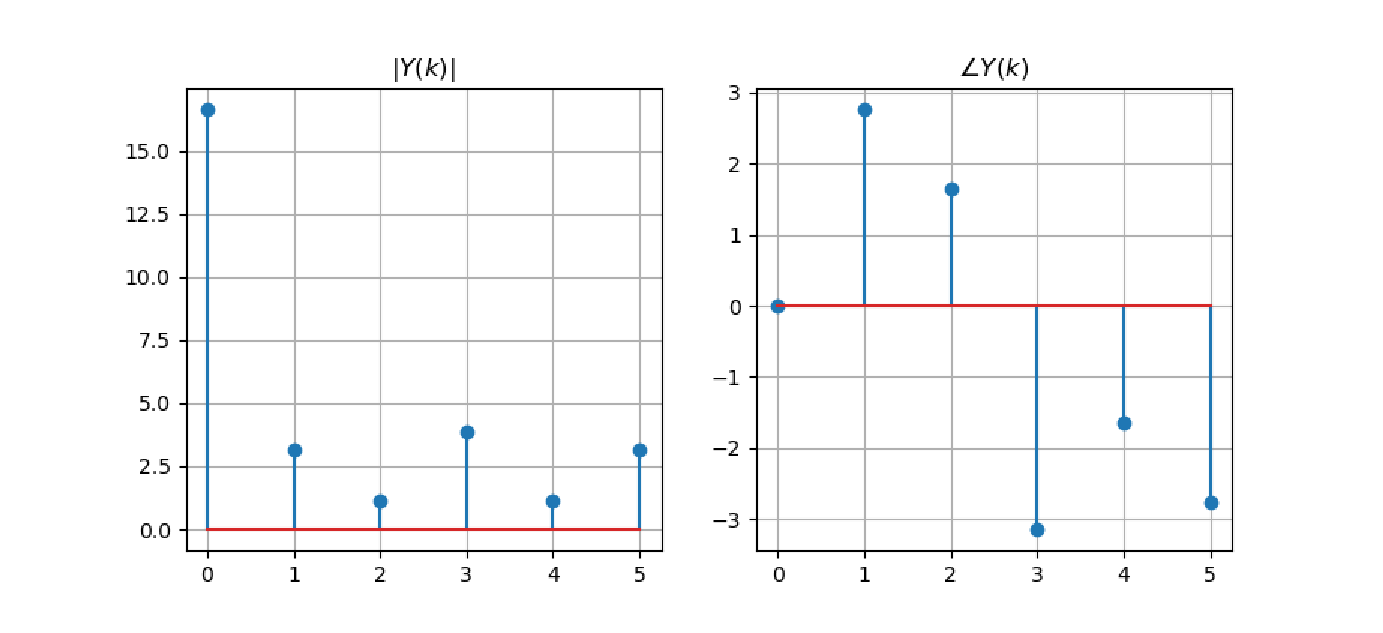
\includegraphics[width=1.15\columnwidth]{./figs/ee18btech11017_fig2.eps}
\end{figure}



\item The following code plots all the above figures.
\begin{lstlisting}
https://github.com/yashwanthguguloth24/EE3025-DSP-lab/tree/main/Assignment1/codes/ee18btech11017_1.py
\end{lstlisting}

%\item Code for Computing DFT of $x(n)$ and $h(n)$
%\solution\\
%Assuming length of $h(n)$ is $250$ for better plotting of Frequency Components.\\
%\newline
%Code is in
%\begin{lstlisting}
%    codes/ee18btech11017.py
%\end{lstlisting}
%Magnitude and Phase Plots of $X(k)$ and $H(k)$

\end{enumerate}

\section{DFT Properties}

\begin{enumerate}[label=\thesection.\arabic*.,ref=\thesection.\theenumi]
\numberwithin{equation}{enumi}

\item \emph{Properties}
\begin{enumerate}
\item Symmetric Property : \[ W^{k+N/2}_{N} = - W^{k}_{N} \] 
\item Periodic Property : \[ W^{k+N}_{N} =  W^{k}_{N} \] 
\item Square Property : \[ W^{2}_{N} =  W_{N/2} \] 
\end{enumerate}


\item For a N-point DFT we can write,
    \begin{align}
        X(k) = \sum_{n=0}^{N-1} x(n)W^{nk}_{N}, \quad k=0,1, \ldots, N-1
    \end{align}

Dividing the inputs into even and odd indices and using Property(c),
    \begin{align}
       X(k) &= \sum_{n=even} x(n)W^{kn}_{N} + \sum_{n=odd} x(n)W^{kn}_{N} \\
       &= \sum_{m=0}^{N/2 -1} x(2m)W^{2mk}_{N} + \sum_{m=0}^{N/2 -1} x(2m+1)W^{(2m+1)k}_{N} \\
       &= \sum_{m=0}^{N/2 -1} x(2m)W^{mk}_{N/2} + W^{k}_{N} \sum_{m=0}^{N/2 -1} x(2m+1)W^{mk}_{N/2} 
    \end{align}
Finally,

\begin{align}
X(k) = \underbrace{X_{e}(k)}_\myText{ N/2 point DFT \\ with even inputs} + W_{N}^k \underbrace{X_{o}(k)}_\myText{N/2 point DFT \\ with odd inputs}
\label{eq:equation3}
\end{align}        
    
Taking N = 6 and expressing the even odd DFT's $X_{e}(k)$ , $X_{o}(k)$ interms of matrices we get,

\begin{equation}
\begin{bmatrix}
X_{e}(0) \\ 
X_{e}(1) \\ 
X_{e}(2) \\ 
X_{o}(0) \\ 
X_{o}(1) \\ 
X_{o}(2)
\end{bmatrix}
=
\begin{bmatrix}
W^{0}_{3} & W^{0}_{3} & W^{0}_{3} & 0 & 0 & 0\\
W^{0}_{3} & W^{1}_{3} & W^{2}_{3} & 0 & 0 & 0\\
W^{0}_{3} & W^{2}_{3} & W^{4}_{3} & 0 & 0 & 0\\
0 & 0 & 0 & W^{0}_{3} & W^{0}_{3} & W^{0}_{3}\\
0 & 0 & 0 & W^{0}_{3} & W^{1}_{3} & W^{2}_{3}\\
0 & 0 & 0 & W^{0}_{3} & W^{2}_{3} & W^{4}_{3}
\end{bmatrix}
\begin{bmatrix}
x(0) \\ 
x(2) \\ 
x(4) \\ 
x(1) \\ 
x(3) \\ 
x(5) 
\end{bmatrix}   
\end{equation}
    
Let, $F_{N}$ be a N-Point DFT Matrix and $P_{N}$ is an odd-even Permutation Matrix, we can write above equation as

\begin{equation}
\begin{bmatrix}
X_{e}(0) \\ 
X_{e}(1) \\ 
X_{e}(2) \\ 
X_{o}(0) \\ 
X_{o}(1) \\ 
X_{o}(2)
\end{bmatrix}
=
\begin{bmatrix}
F_{3} & 0 \\
0 & F_{3}
\end{bmatrix}
P_{6}
x   
\label{eq:equation6}
\end{equation}


where
\begin{equation}
P_{6} 
=
\begin{bmatrix}
1 & 0 & 0 & 0 & 0 & 0\\
0 & 0 & 1 & 0 & 0 & 0\\
0 & 0 & 0 & 0 & 1 & 0\\
0 & 1 & 0 & 0 & 0 & 0\\
0 & 0 & 0 & 1 & 0 & 0\\
0 & 0 & 0 & 0 & 0 & 1
\end{bmatrix} 
\end{equation}

and 
\begin{equation}
P_{6}x
=
P_{6}
\begin{bmatrix}
x(0) \\ 
x(1) \\ 
x(2) \\ 
x(3) \\ 
x(4) \\ 
x(5) 
\end{bmatrix}
=
\begin{bmatrix}
x(0) \\ 
x(2) \\ 
x(4) \\ 
x(1) \\ 
x(3) \\ 
x(5) 
\end{bmatrix}   
\end{equation}

Now,using \eqref{eq:equation3} we can express $X(k)$ interms of $X_{e}(k)$ and $X_{o}(k)$

\begin{equation}
\begin{bmatrix}
X(0) \\ 
X(1) \\ 
X(2) \\ 
X(3) \\ 
X(4) \\ 
X(5) 
\end{bmatrix}
=
\begin{bmatrix}
1 & 0 & 0 & W^{0}_{6} & 0 & 0\\
0 & 1 & 0 &  0 & W^{1}_{6} & 0\\
0 & 0 & 1 & 0 & 0 & W^{2}_{6}\\
1 & 0 & 0 & W^{3}_{6} & 0 & 0\\
0 & 1 & 0 & 0 & W^{4}_{6} & 0\\
0 & 0 & 1 & 0 & 0 & W^{5}_{6}
\end{bmatrix}
\begin{bmatrix}
X_{e}(0) \\ 
X_{e}(1) \\ 
X_{e}(2) \\ 
X_{o}(0) \\ 
X_{o}(1) \\ 
X_{o}(2)
\end{bmatrix}
\label{eq:equation4}
\end{equation}


Considering $I_{3}$ to be 3x3 identity matrix and $D_{N} = diag(1,W_{N},W_{N}^{2},....,W_{N}^{N-1})$ . So that $D_{\frac{N}{2}} = diag(1,W_{N},W_{N}^{2},....,W_{N}^{\frac{N}{2} -1})$. Therefore $D_{3}$ will be,
\begin{equation}
D_{3}=
\begin{bmatrix}
1 & 0 & 0 \\
0 & W^{1}_{6} & 0 \\
0 & 0 & W^{2}_{6}
\end{bmatrix}
\end{equation}

Using Property(a), Equation \eqref{eq:equation4} and above defined $D_{3}$ and $I_{3}$ we can write,

\begin{equation}
X
=
\begin{bmatrix}
X(0) \\ 
X(1) \\ 
X(2) \\ 
X(3) \\ 
X(4) \\ 
X(5) 
\end{bmatrix}
=
\begin{bmatrix}
I_{3} & D_{3} \\
I_{3} & -D_{3}
\end{bmatrix}
\begin{bmatrix}
X_{e}(0) \\ 
X_{e}(1) \\ 
X_{e}(2) \\ 
X_{o}(0) \\ 
X_{o}(1) \\ 
X_{o}(2)
\end{bmatrix}
\label{eq:equation5}
\end{equation}

Finally using Eq \eqref{eq:equation5} and Eq \eqref{eq:equation6} we get


\begin{equation}
X
=
\begin{bmatrix}
I_{3} & D_{3} \\
I_{3} & -D_{3}
\end{bmatrix}
\begin{bmatrix}
F_{3} & 0 \\
0 & F_{3}
\end{bmatrix}
P_{6}
x 
\label{eq:equation7}
\end{equation}

Using $X = F_{6}x$ for N = 6;
\begin{equation}
\implies 
F_{6}
=
\begin{bmatrix}
I_{3} & D_{3} \\
I_{3} & -D_{3}
\end{bmatrix}
\begin{bmatrix}
F_{3} & 0 \\
0 & F_{3}
\end{bmatrix}
P_{6}
\end{equation}

Therefore, for an arbitary $N$ we can express N-point DFT Matrix in terms of N/2-point DFT Matrix as

\begin{equation} 
F_{N}
=
\begin{bmatrix}
I_{N/2} & D_{N/2} \\
I_{N/2} & -D_{N/2}
\end{bmatrix}
\begin{bmatrix}
F_{N/2} & 0 \\
0 & F_{N/2}
\end{bmatrix}
P_{N}
\label{eq:equation8}
\end{equation}

\item Now, if $N = 2^{M}$ where $M \in \mathbb{Z^{+}}$  then we can recursively breakdown N/2 point DFT Matrix to N/4 point DFT Matrix ..so on till we reach 2-point DFT Matrix.So for N = 8, using Eq \eqref{eq:equation8} we can write,

\begin{equation}
F_{8}=
\begin{bmatrix}
I_{4} & D_{4} \\
I_{4} & -D_{4}
\end{bmatrix}
\begin{bmatrix}
F_{4} & 0 \\
0 & F_{4}
\end{bmatrix}
P_{8}
\end{equation}
\begin{equation}
F_{4}=
\begin{bmatrix}
I_{2} & D_{2} \\
I_{2} & -D_{2}
\end{bmatrix}
\begin{bmatrix}
F_{2} & 0 \\
0 & F_{2}
\end{bmatrix}
P_{4}
\end{equation}

Finally, the 2-point DFT Matrix is the base case 
\begin{equation}
F_{2}
\begin{bmatrix}
x_{1} \\
x_{2}
\end{bmatrix}
=
\begin{bmatrix}
1 & 1 \\
1 & -1
\end{bmatrix}
\begin{bmatrix}
x_{1} \\
x_{2}
\end{bmatrix}
=
\begin{bmatrix}
x_{1}+x_{2} \\
x_{1}-x_{2}
\end{bmatrix}
\end{equation}


\item Step by Step visualization of computing 8-Point DFT recursively using 4-point DFT's and 2-point DFT's.Expressing 8-point DFT's in terms of 4-point DFT's.
\begin{equation}
\begin{bmatrix}
X(0) \\ 
X(1) \\ 
X(2) \\ 
X(3)
\end{bmatrix}
=
\begin{bmatrix}
X_{e}(0) \\ 
X_{e}(1)\\ 
X_{e}(2)\\
X_{e}(3)\\
\end{bmatrix}
+
\begin{bmatrix}
W^{0}_{8} & 0 & 0 & 0\\
0 & W^{1}_{8} & 0 & 0\\
0 & 0 & W^{2}_{8} & 0\\
0 & 0 & 0 & W^{3}_{8}
\end{bmatrix}
\begin{bmatrix}
X_{o}(0) \\ 
X_{o}(1) \\ 
X_{o}(2) \\
X_{o}(3)
\end{bmatrix}
\end{equation}

\begin{equation}
\begin{bmatrix}
X(4) \\ 
X(5) \\ 
X(6) \\ 
X(7)
\end{bmatrix}
=
\begin{bmatrix}
X_{e}(0) \\ 
X_{e}(1)\\ 
X_{e}(2)\\
X_{e}(3)\\
\end{bmatrix}
-
\begin{bmatrix}
W^{0}_{8} & 0 & 0 & 0\\
0 & W^{1}_{8} & 0 & 0\\
0 & 0 & W^{2}_{8} & 0\\
0 & 0 & 0 & W^{3}_{8}
\end{bmatrix}
\begin{bmatrix}
X_{o}(0) \\ 
X_{o}(1) \\ 
X_{o}(2) \\
X_{o}(3)
\end{bmatrix}
\end{equation}

Now, 4-point DFT's to 2-point DFT's
\begin{equation}
\begin{bmatrix}
X_{e}(0) \\ 
X_{e}(1)\\ 
\end{bmatrix}
=
\begin{bmatrix}
X_{e_{1}}(0) \\ 
X_{e_{1}}(1)\\ 
\end{bmatrix}
+
\begin{bmatrix}
W^{0}_{4} & 0\\
0 & W^{1}_{4}
\end{bmatrix}
\begin{bmatrix}
X_{o_{1}}(0) \\ 
X_{o_{1}}(1) \\ 
\end{bmatrix}
\end{equation}
\begin{equation}
\begin{bmatrix}
X_{e}(2) \\ 
X_{e}(3)\\ 
\end{bmatrix}
=
\begin{bmatrix}
X_{e_{1}}(0) \\ 
X_{e_{1}}(1)\\ 
\end{bmatrix}
-
\begin{bmatrix}
W^{0}_{4} & 0\\
0 & W^{1}_{4}
\end{bmatrix}
\begin{bmatrix}
X_{o_{1}}(0) \\ 
X_{o_{1}}(1) \\ 
\end{bmatrix}
\end{equation}

\begin{equation}
\begin{bmatrix}
X_{o}(0) \\ 
X_{o}(1)\\ 
\end{bmatrix}
=
\begin{bmatrix}
X_{e_{2}}(0) \\ 
X_{e_{2}}(1)\\ 
\end{bmatrix}
+
\begin{bmatrix}
W^{0}_{4} & 0\\
0 & W^{1}_{4}
\end{bmatrix}
\begin{bmatrix}
X_{o_{2}}(0) \\ 
X_{o_{2}}(1) \\ 
\end{bmatrix}
\end{equation}
\begin{equation}
\begin{bmatrix}
X_{o}(2) \\ 
X_{o}(3)\\ 
\end{bmatrix}
=
\begin{bmatrix}
X_{e_{2}}(0) \\ 
X_{e_{2}}(1)\\ 
\end{bmatrix}
-
\begin{bmatrix}
W^{0}_{4} & 0\\
0 & W^{1}_{4}
\end{bmatrix}
\begin{bmatrix}
X_{o_{2}}(0) \\ 
X_{o_{2}}(1) \\ 
\end{bmatrix}
\end{equation}
\begin{equation}
P_{8}
\begin{bmatrix}
x(0) \\ 
x(1) \\ 
x(2) \\ 
x(3) \\ 
x(4) \\ 
x(5) \\
x(6) \\
x(7)
\end{bmatrix}
 = 
\begin{bmatrix}
x(0) \\ 
x(2) \\ 
x(4) \\ 
x(6) \\
x(1) \\ 
x(3) \\ 
x(5) \\
x(7)
\end{bmatrix}
\end{equation}

\begin{equation}
P_{4}
\begin{bmatrix}
x(0) \\ 
x(2) \\ 
x(4) \\ 
x(6) \\
\end{bmatrix}
 = 
\begin{bmatrix}
x(0) \\ 
x(4) \\ 
x(2) \\
x(6)
\end{bmatrix}
\end{equation}
\begin{equation}
P_{4}
\begin{bmatrix}
x(1) \\ 
x(3) \\ 
x(5) \\
x(7)
\end{bmatrix}
 = 
\begin{bmatrix}
x(1) \\ 
x(5) \\ 
x(3) \\ 
x(7) \\
\end{bmatrix}
\end{equation}

Finally,

\begin{equation}
\begin{bmatrix}
X_{e_{1}}(0) \\ 
X_{e_{1}}(1)\\ 
\end{bmatrix}
= F_{2}
\begin{bmatrix}
x(0) \\ 
x(4) \\ 
\end{bmatrix}
=
\begin{bmatrix}
x(0)+x(4) \\ 
x(0)-x(4) \\ 
\end{bmatrix}
\end{equation}
\begin{equation}
\begin{bmatrix}
X_{o_{1}}(0) \\ 
X_{o_{1}}(1)\\ 
\end{bmatrix}
= F_{2}
\begin{bmatrix}
x(2) \\ 
x(6) \\ 
\end{bmatrix}
=
\begin{bmatrix}
x(2)+x(6) \\ 
x(2)-x(6) \\ 
\end{bmatrix}
\end{equation}
\begin{equation}
\begin{bmatrix}
X_{e_{2}}(0) \\ 
X_{e_{2}}(1)\\ 
\end{bmatrix}
= F_{2}
\begin{bmatrix}
x(1) \\ 
x(5) \\ 
\end{bmatrix}
=
\begin{bmatrix}
x(1)+x(5) \\ 
x(1)-x(5) \\ 
\end{bmatrix}
\end{equation}
\begin{equation}
\begin{bmatrix}
X_{o_{2}}(0) \\ 
X_{o_{2}}(1)\\ 
\end{bmatrix}
= F_{2}
\begin{bmatrix}
x(3) \\ 
x(7) \\ 
\end{bmatrix}
=
\begin{bmatrix}
x(3)+x(7) \\ 
x(3)-x(7) \\ 
\end{bmatrix}
\end{equation}


So, $X_{e_{2}} \in \text{DFT} \{x(1),x(5)\}$ and $X_{o_{2}} \in \text{DFT} \{x(3),x(7)\}$ would combine to give $X_{o}$ .And $X_{e_{1}} \in \text{DFT} \{x(0),x(4)\}$ and $X_{o_{1}} \in \text{DFT} \{x(2),x(6)\}$ would combine to give $X_{e}$.



\item \emph{Time Complexity:} \\
In DFT - Matrix multiplication of NxN matrix with Nx1 vector.
Hence it has $O(N^2)$ time complexity which is very slow for high $N$.
\newline
In this recursive approach which is termed as FFT - N-point FFT is broken down recursively into 2 N/2-point FFTs recursively.
Additionally $O(N)$ operation of Vector multiplication is performed on the N/2 point FFTs.
\begin{equation}
    T(n) = 2T(n/2) + O(n)
\end{equation}
Solving this recurrence relation gives $O(NlogN)$ time complexity.

\item Computing $X(k)$, $H(k)$ and $Y(k)$ for 
    \begin{align}
        x(n) = \cbrak{\underset{\uparrow}{1},2,3,4,2,1,0,0}
    \end{align}
with N = 8, using above FFT approach.

\begin{figure}[!ht]
	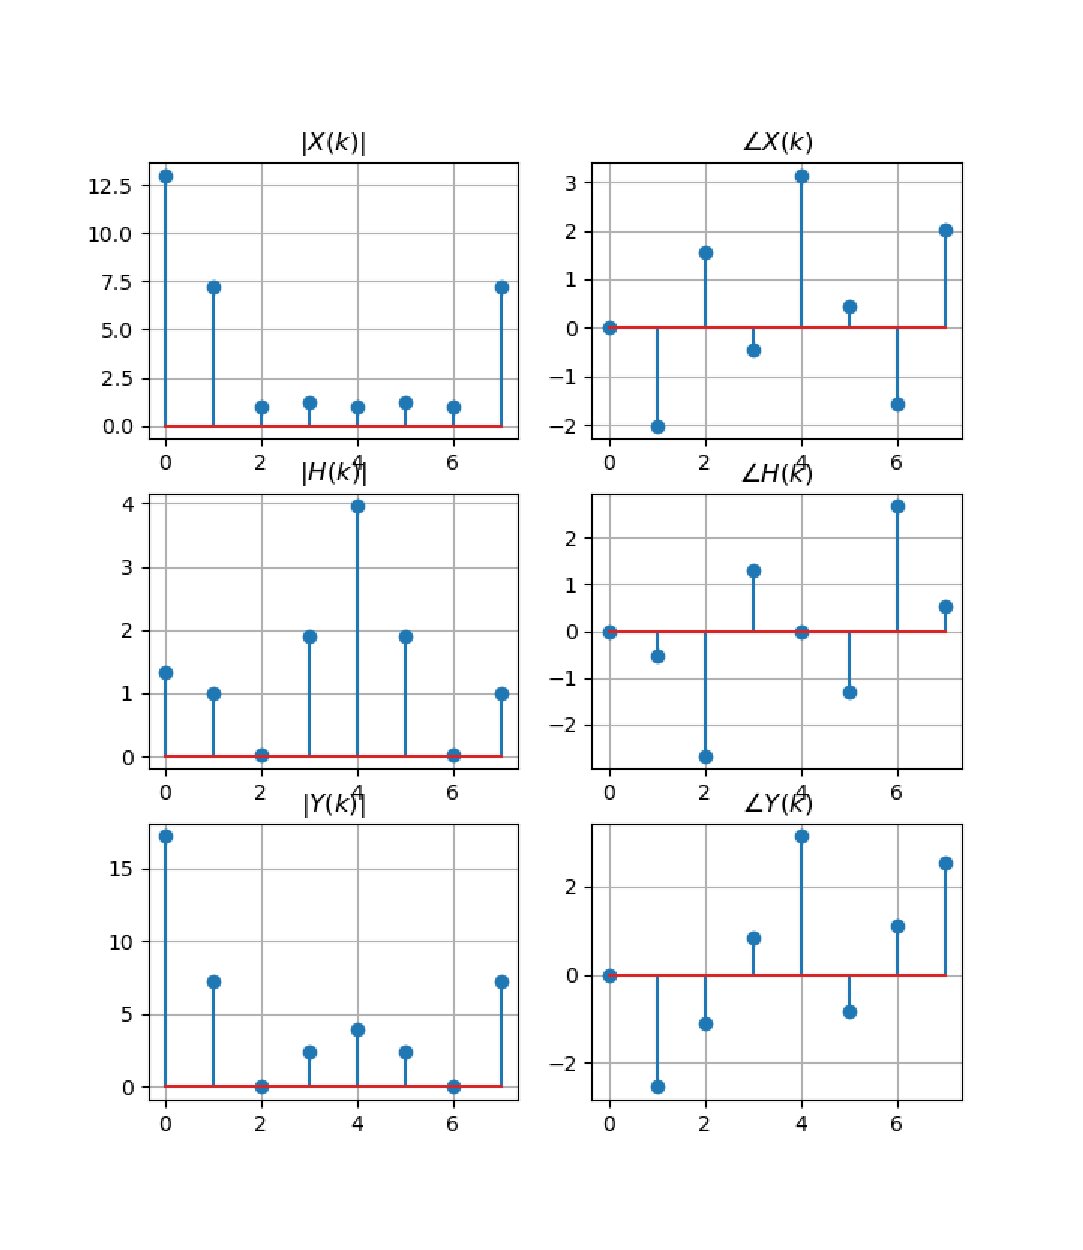
\includegraphics[width=1.15\columnwidth]{./figs/ee18btech11017_fig3.eps}
\end{figure}
We can observe that both the approaches produces that same plots.

\item The following code plots magnitude and phase plots of $X(k)$, $H(k)$ and $Y(k)$ .
\begin{lstlisting}
https://github.com/yashwanthguguloth24/EE3025-DSP-lab/tree/main/Assignment1/codes/ee18btech11017_2.py
\end{lstlisting}


\item \emph{Computation Times:} \\
We can compare the computation times for DFT,FFT and Inbuit-FFT algorithms for N = $2^{M}$, for N = 1 ($2^{0}$) to 8192 ($2^{13}$).

\begin{figure}[!ht]
	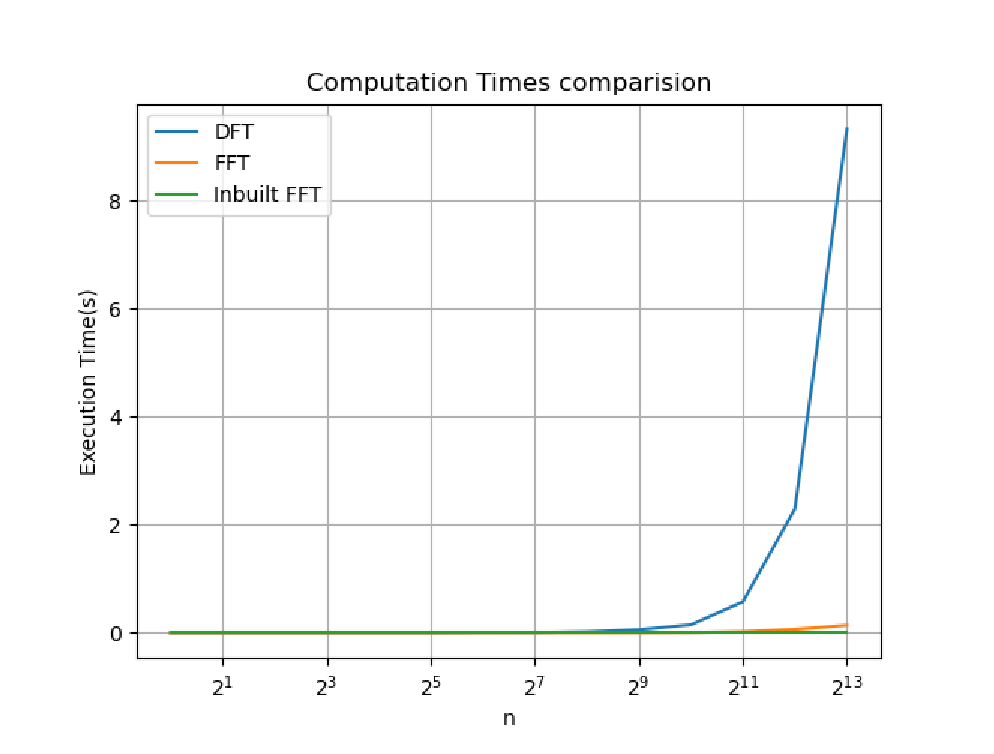
\includegraphics[width=1.15\columnwidth]{./figs/ee18btech11017_fig4.eps}
\end{figure}

From above plot we can observe that, computation time for DFT rises exponentially as we increase N in powers of 2 but FFT and Inbuilt-FFT are much faster.

\item The following code plots the above time comparision plot.
\begin{lstlisting}
https://github.com/yashwanthguguloth24/EE3025-DSP-lab/tree/main/Assignment1/codes/ee18btech11017_3.py
\end{lstlisting}


\end{enumerate}

























\end{document}
